%"###############################################
%
% Classification RTUPB pre 
%
%###############################################

\begin{figure}[H]
\centering
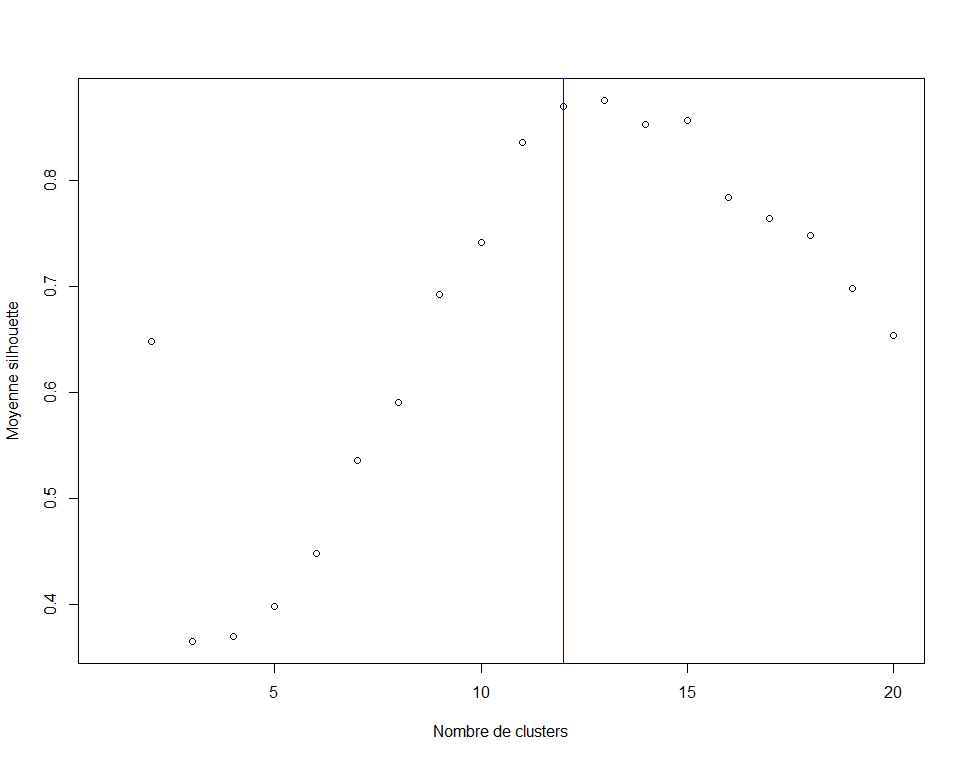
\includegraphics[width=0.90\textwidth]{../Fig/RTUPB/rtupb-elbow-pre.png}
\caption{RTUPB Maximise nb cluster / bonne classification}
\end{figure}

\begin{figure}[H]
\centering
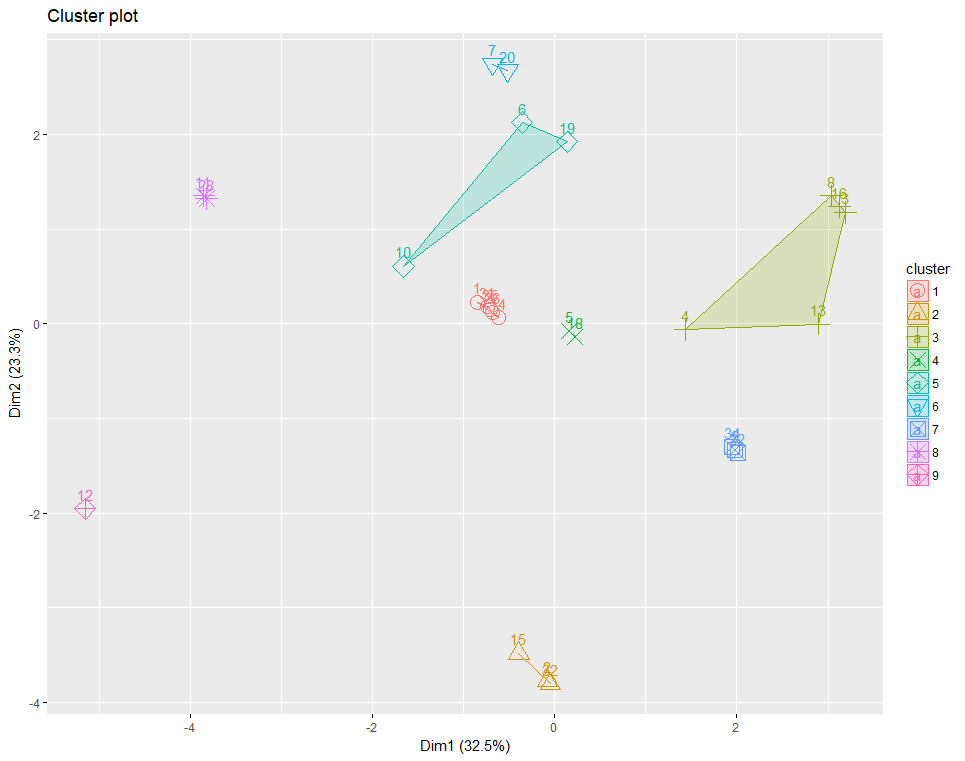
\includegraphics[width=0.90\textwidth]{../Fig/RTUPB/rtupb-pam-k12.png}
\caption{RTUPB Nuage de points / clusters PAM k=12 }
\end{figure}

\begin{figure}[H]
\centering
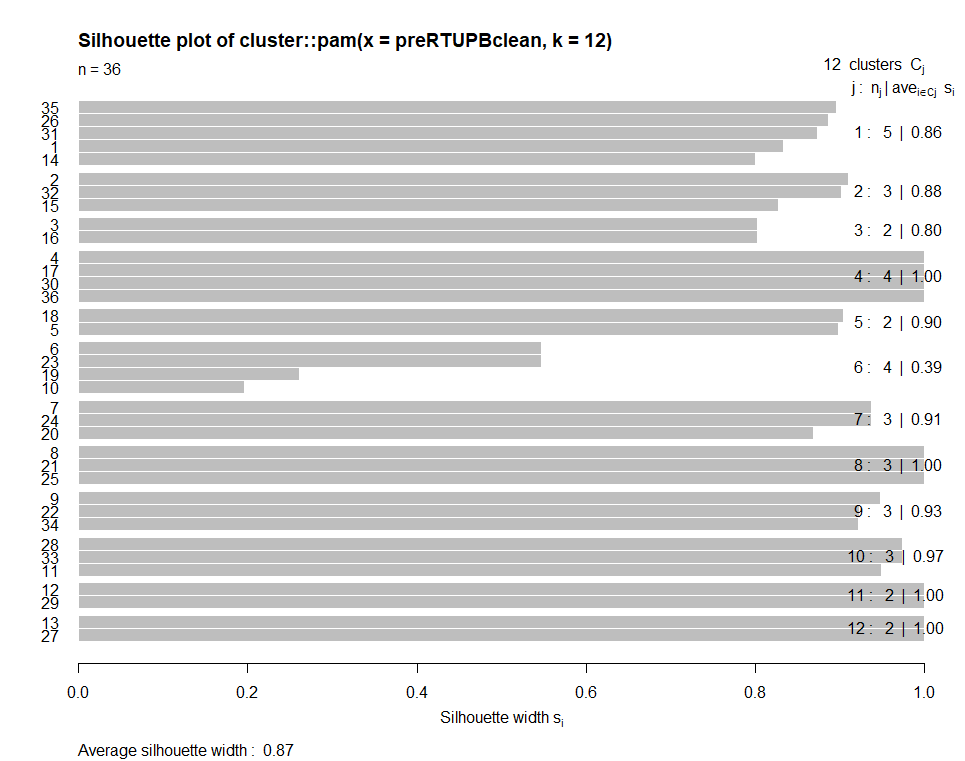
\includegraphics[width=0.90\textwidth]{../Fig/RTUPB/rtupb-sil-k12-pre.png}
\caption{RTUPB Nuage de points / clusters PAM k=12 }
\end{figure}

\begin{figure}[H]
\centering
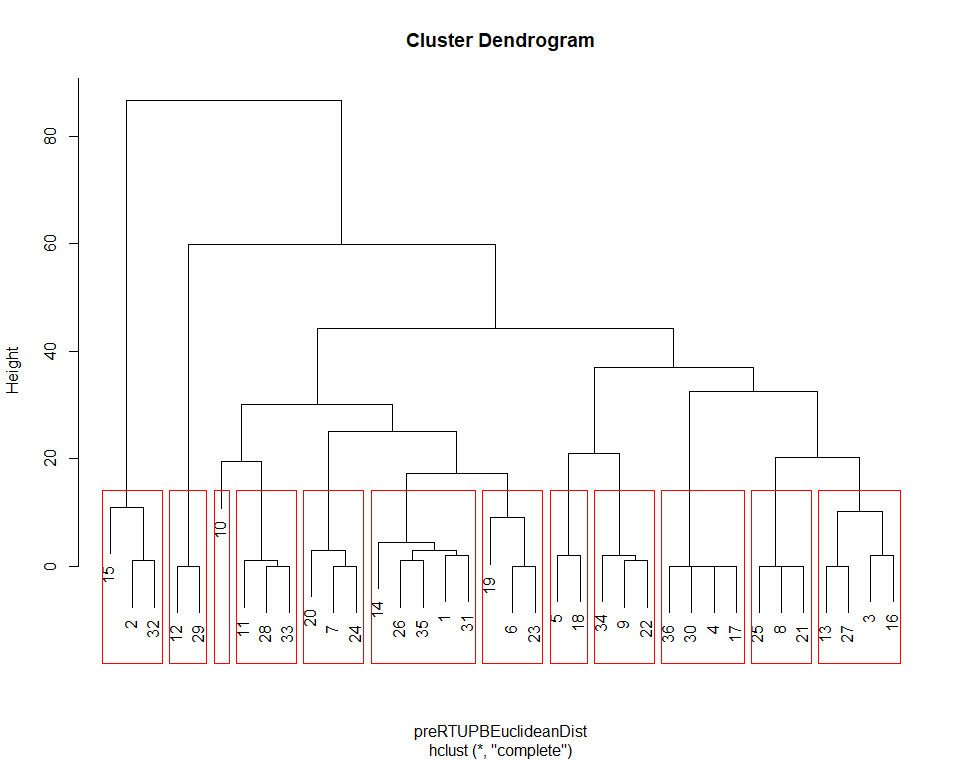
\includegraphics[width=0.90\textwidth]{../Fig/RTUPB/rtupb-cah-k12-pre.png}
\caption{RTUPB CAH séparation en k=12 }
\end{figure}


%"###############################################
%
% Interpretation des trois figures RTUPB pre 
%
%#############################################

Lors de notre analyse nous avons observé qu'il existait un ensemble d'individus similaires (ensemble des valeurs
identiques au relevé prés) ce qui s'observer dans la construction de certains clusters avec une valeur de qualité 
intra-cluster très forte en forgeant de petit clusters. Nous reviendrons sur ce point dans le rapprochement de ces
profils avec les profils de guérison ultérieurement. Nous avons estimé à 12 le nombre de clusters suivant la variation 
de la qualité globale  du cluster réalisé à partir de PAM. 



%\begin{figure}[h]
%    \begin{minipage}[c]{.46\linewidth}
%        \centering
%        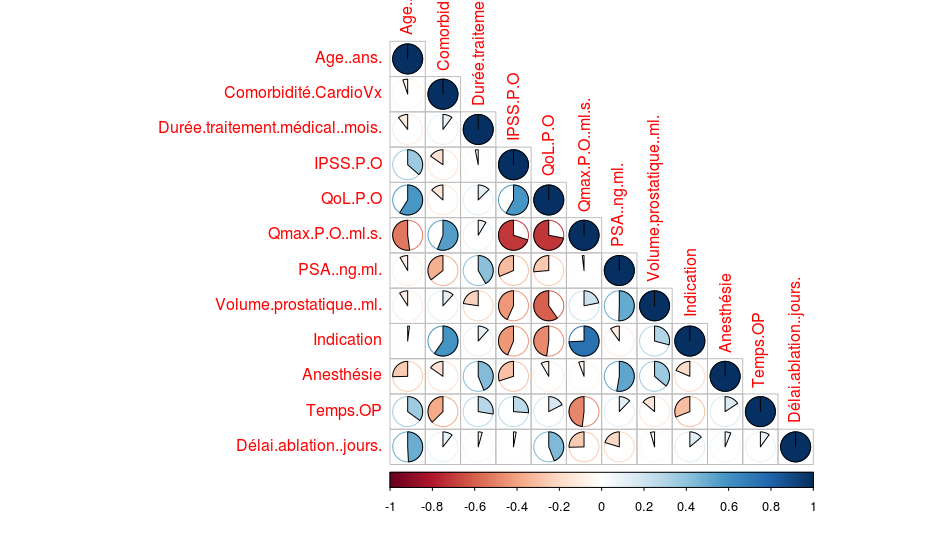
\includegraphics[width=1\textwidth]{../Fig/VPPBS/vppbs-corr-matrice-pie}
%        \caption{Légende}
%    \end{minipage}
%    \hfill%
%    \begin{minipage}[c]{.46\linewidth}
%        \centering
%        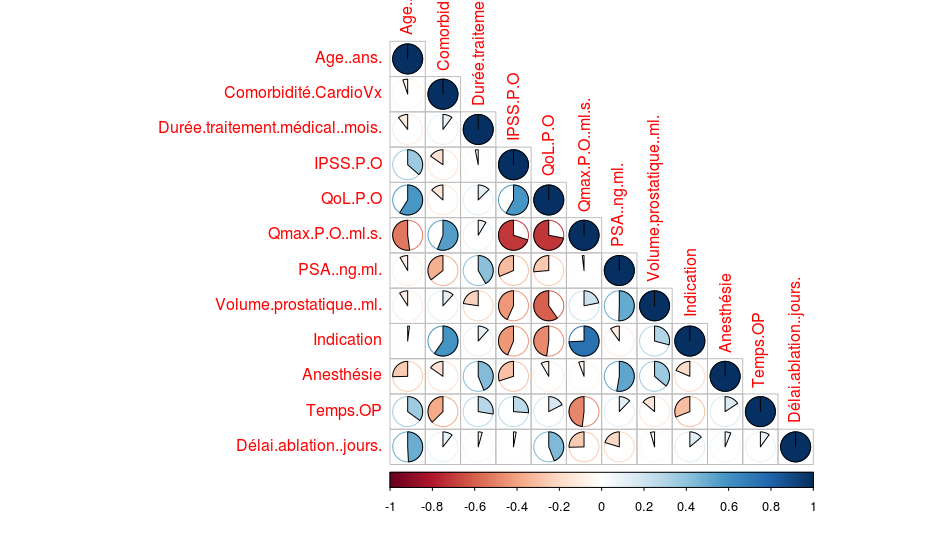
\includegraphics[width=1\textwidth]{../Fig/VPPBS/vppbs-corr-matrice-pie}
%        \caption{Légende}
%    \end{minipage}
%\end{figure}





%
%##########################
%# CONCLUSION
%##########################
